%Part of/Parte di https://github.com/f-dinucci/appuntiMeccanicaFluidi/
%License/Licenza Creative Commons Attribution-ShareAlike 4.0 International (CC BY-SA 4.0) - attribution/attribuzione Francesco Di Nucci
%See also/Vedere anche https://creativecommons.org/licenses/by-sa/4.0/ and/e https://creativecommons.org/licenses/by-sa/4.0/legalcode
%
\section{Spinte sulle superfici}
Ricordando che in un fluido statico è presente solo lo sforzo normale (alias la pressione), questo esercita sulle superfici a contatto con il fluido una forza detta spinta idrostatica o spinta.
Questa forza può ovviamente generare un momento statico.

\subsection{Forze e momenti}
Ricordando che in un sistema discreto si ha:
	\begin{equation*}
		\begin{gathered}
			\text{Forza} \quad \uline{F} = \sum_i \uline{F}_i \\
			\text{Coppia} \quad \uline{M} = \sum \uline{r}_i \cross \uline{F}_i
		\end{gathered}
	\end{equation*}
Per un sistema continuo come ad esempio quello di fig. 2.1, si può scrivere l'analogo:
	\begin{equation*}
		\begin{gathered}
			\text{Dato che in generale per la pressione}\\
			\uline{F} = \int \uuline{J}_Q \vdot \uline{n} \dd{S} = \int p \uline{n} \dd{S}\\
			\text{dato che sul sistema agisce anche la pressione atmosferica $p_0$}\\
			\text{Forza} \quad \uline{F}_S =\int_S (p - p_0) \uline{n} \dd{S} = \int_S \rho g (z_0 - z) \uline{n} \dd{S} \\
			\text{Coppia} \quad \uline{M} = \int_S \uline{r} \cross [(p - p_0) \uline{n}]=\int_S (\uline{r} \cross \uline{n}) (p - p_0) \dd{S}
		\end{gathered}
	\end{equation*}
Dove $\uline{r}$, vettore posizione, è la variabile di integrazione, dato che si sta integrando su una superficie.

È come se la forza fosse un vettore di direzione $\uline{n}$ e modulo $(p - p_0) \dd{S}$ e la coppia un vettore di direzione $\uline{r} \cross \uline{n}$ e modulo $(p - p_0) \dd{S}$.

\subsection{Superficie piana verticale}
Il primo caso da analizzare, più semplice, è quello di una superficie piana verticale. La normale alla superficie è la stessa del flusso, dato che un piano ha una sola direzione normale, ed è costante:
	\begin{equation*}
		\uline{F}_S = \int_S \rho g (z_0 - z) \uline{n} \dd{S} = \uline{n} \rho g \int_S (z_0 - z) \dd{S}
	\end{equation*}
Data la disposizione degli assi in figura 2.9, la superficie è verticale, solamente $F_x \neq 0$
	\begin{equation*}
		\begin{gathered}
			F_x = \rho g \int_S (z_0 -z) \dd{y} \dd{z} \\
			F_y = 0 \\
			F_z = 0
		\end{gathered}
	\end{equation*}
	\begin{figure}[h]
		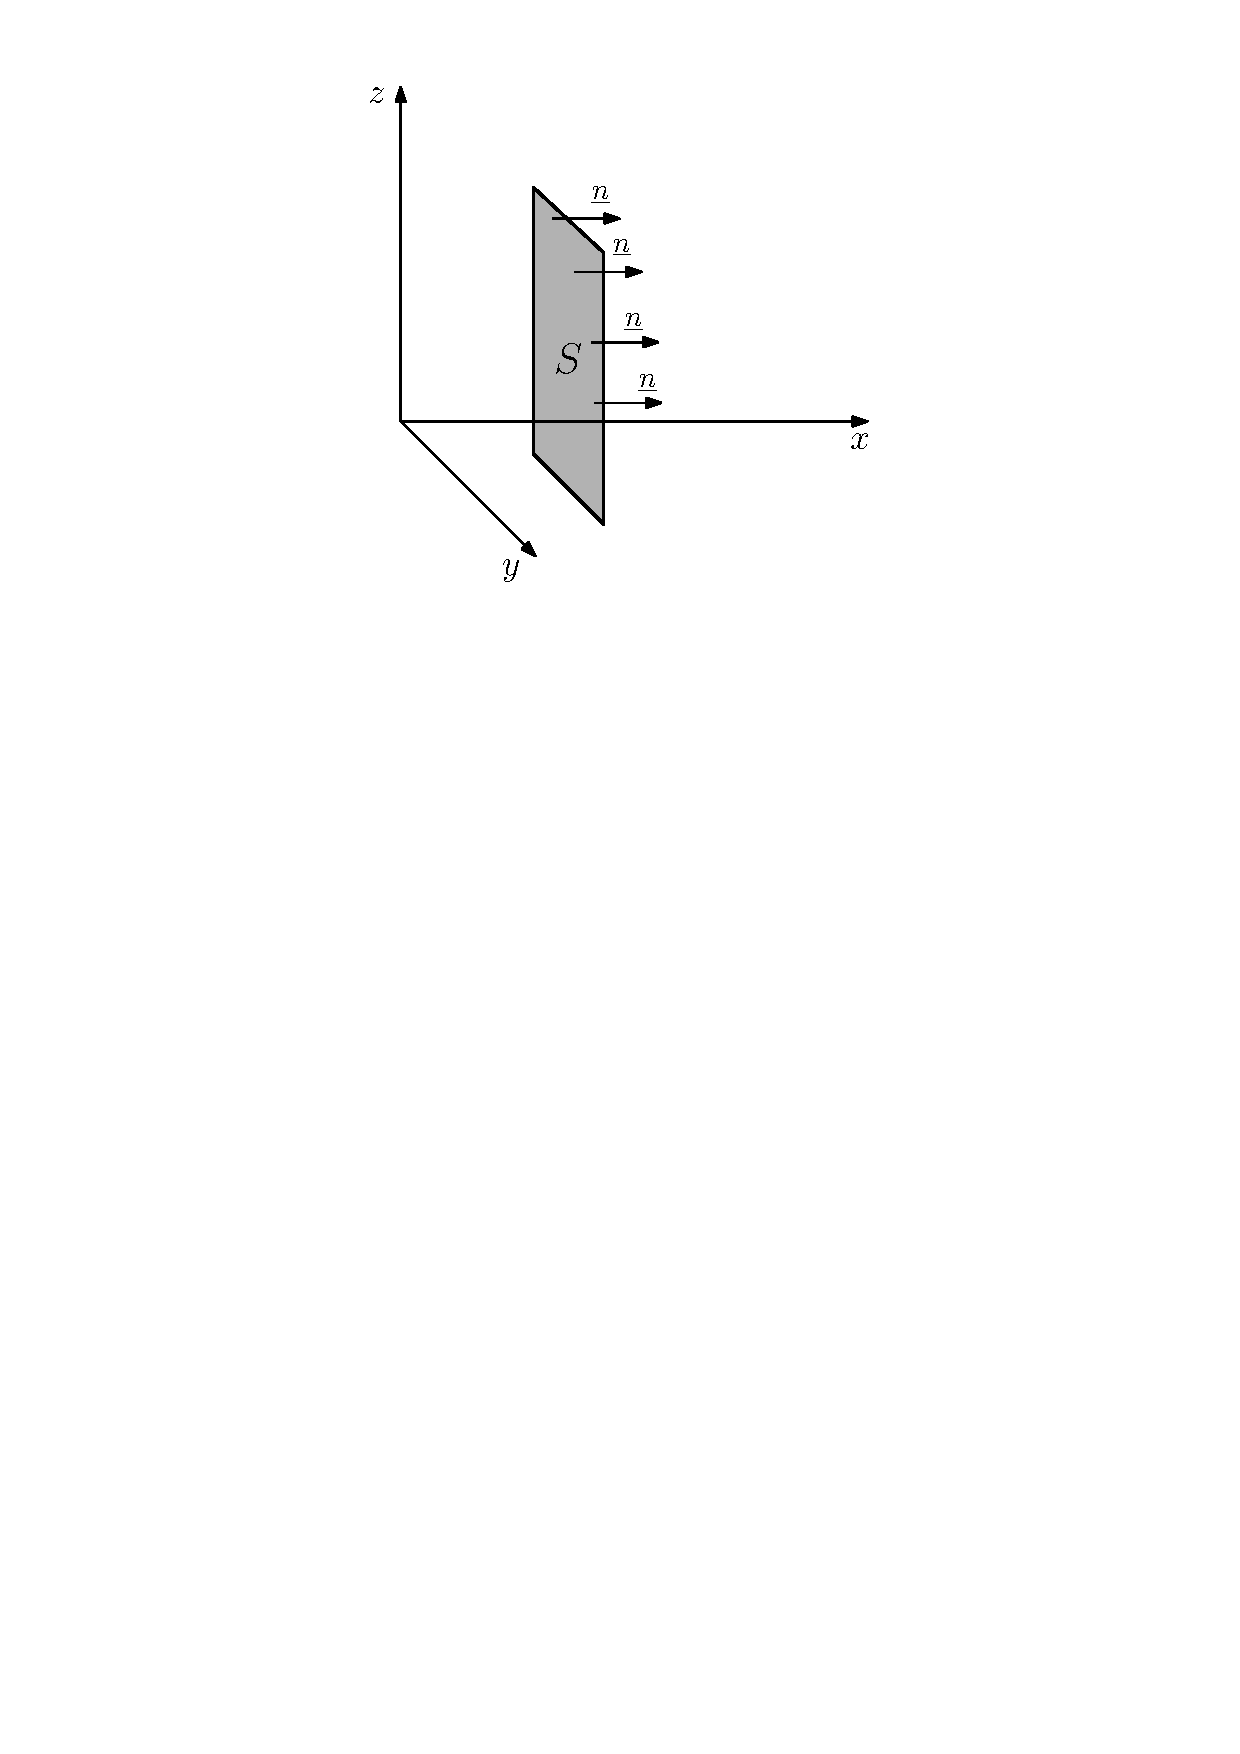
\includegraphics[scale=0.80]{./2.4 Spinte sulle superfici/2.4-1}
		\centering
		\caption{La direzione della forza è nota, ne va calcolato solo il modulo}
	\end{figure}
Il risultato dipende solamente dalla forma della superficie, da un punto di vista matematico l'integrale è equivalente al procedimento di definizione di un baricentro da un punto di vista geometrico\footnote{da non confondersi col baricentro come punto di applicazione della forza di gravità, in questi casi il punto di applicazione differisce dal baricentro}:
	\begin{equation*}
		\begin{gathered}
			x_b = \frac{1}{S} \int x \dd{S} \quad \text{cioè media della x} \\
			y_b = \frac{1}{S} \int y \dd{S} \quad \text{cioè media della y} \\
			z_b = \frac{1}{S} \int z \dd{S} \quad \text{cioè media della z} \\
			\text{da cui nel caso di superficie piana verticale, dato che $\int z \dd{S} = S z_B$} \\
			F_x = \rho g S (z_0 - z_b)
		\end{gathered}
	\end{equation*}
Si ha quindi una interessante correlazione tra la forza su una superficie S ed il baricentro di questa, utile se il baricentro b è noto. Un altro modo di esprimere questa formula è il seguente:
	\begin{equation*}
		F_x = S (p_0 - p_b)\footnote{che è la pressione relativa nel baricentro}
	\end{equation*}
Cioè nel caso di superficie piana verticale, la forza agente è la stessa che si otterrebbe se su tutta la superficie la pressione fosse uguale a quella nel baricentro.
%
\subsection{Superficie piana inclinata e punto di applicazione}
Il caso immediatamente successivo è quello di una superficie piana inclinata.
In questo caso la normale non è parallela ad un asse ma è comunque costante, quindi come prima l'integrale definisce ancora un baricentro.
	\begin{figure}[ht]
		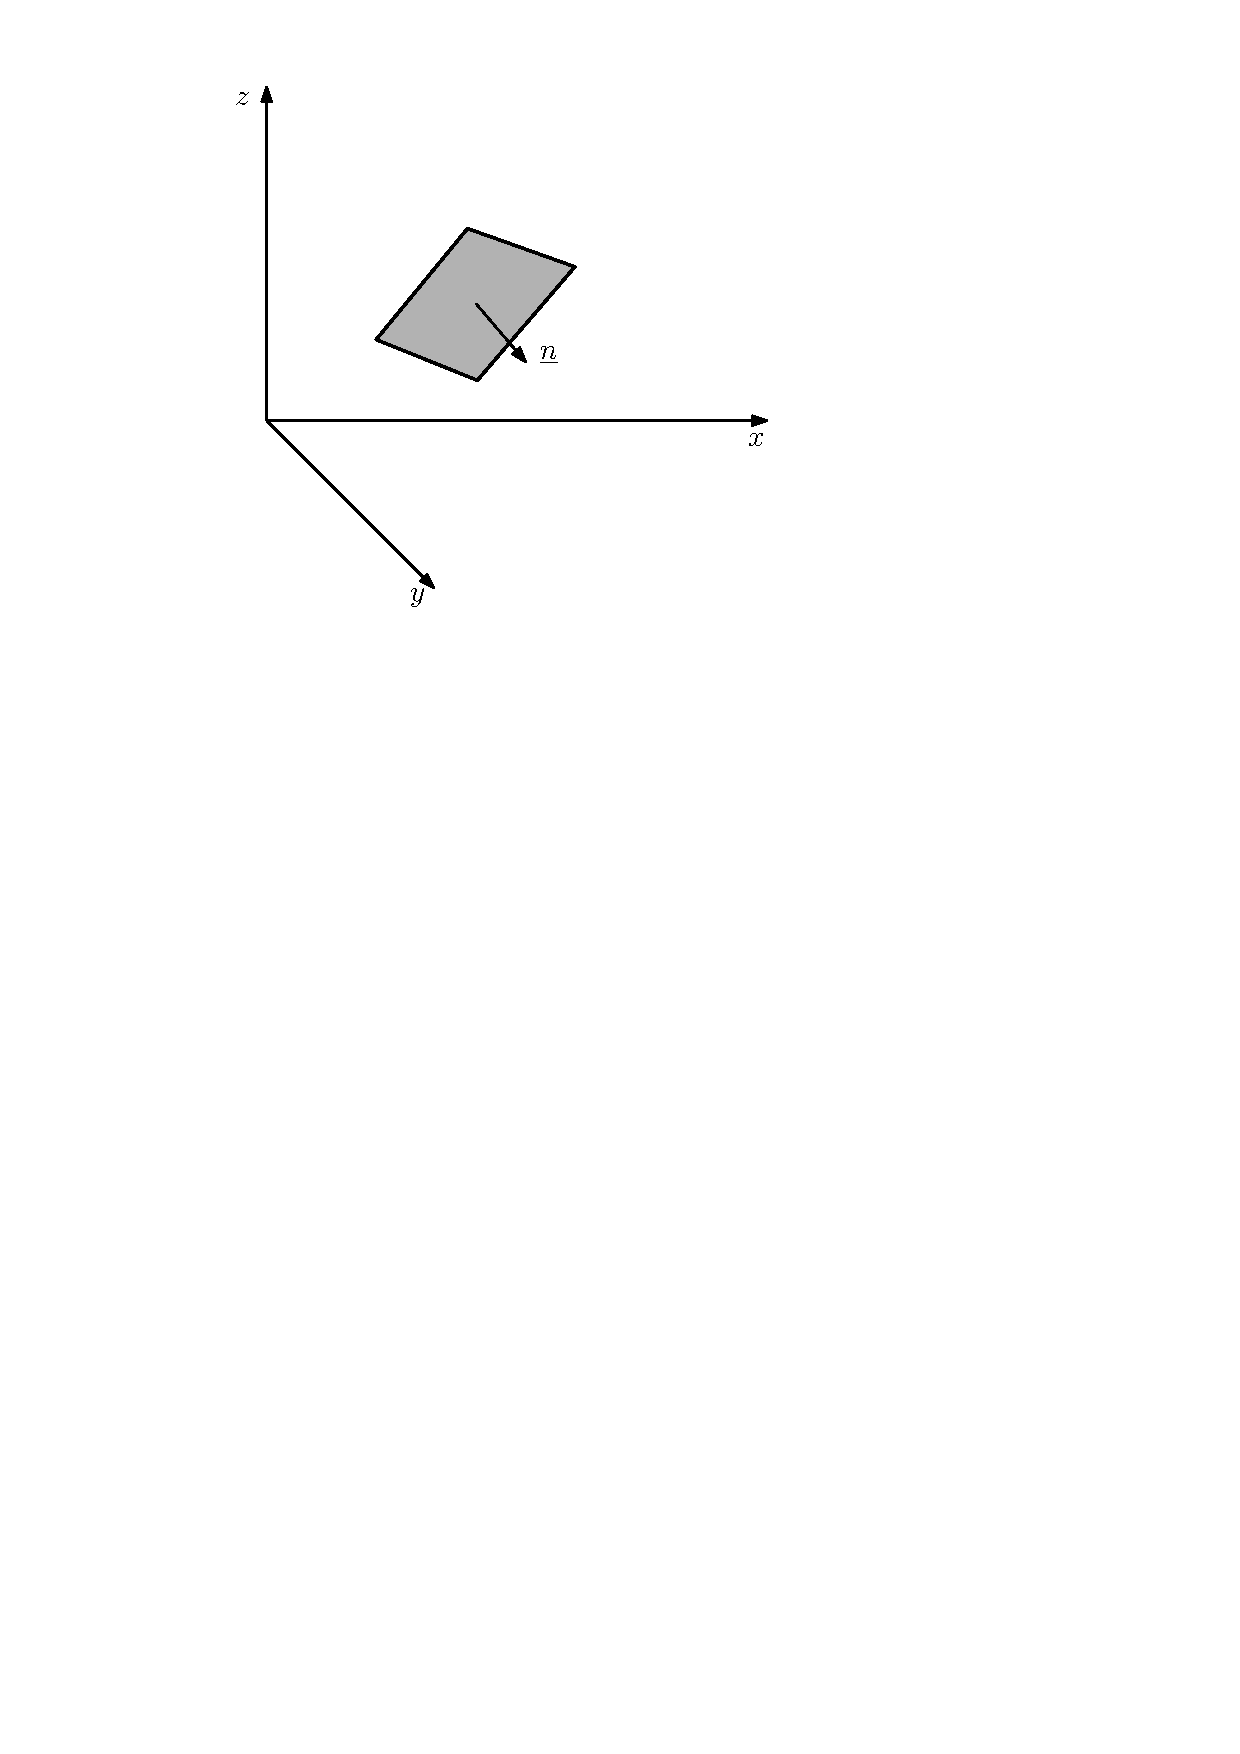
\includegraphics[scale=0.75]{./2.4 Spinte sulle superfici/2.4-2}
		\centering
		\caption{La normale è lungo un piano qualsiasi}
	\end{figure}
Quindi vale ancora l'equivalenza seguente, anche se occorre tener conto della possibilità di componenti della forza su diversi assi:
	\begin{equation*}
		F = S (p_0 - p_b)
	\end{equation*}

Si veda ad esempio il caso di un contenitore pieno d'acqua, con il pelo libero ad altezza $h$, in figura 2.11.
Si può calcolare la forza agente su una delle pareti laterali in modi differenti.
	\begin{figure}[ht]
		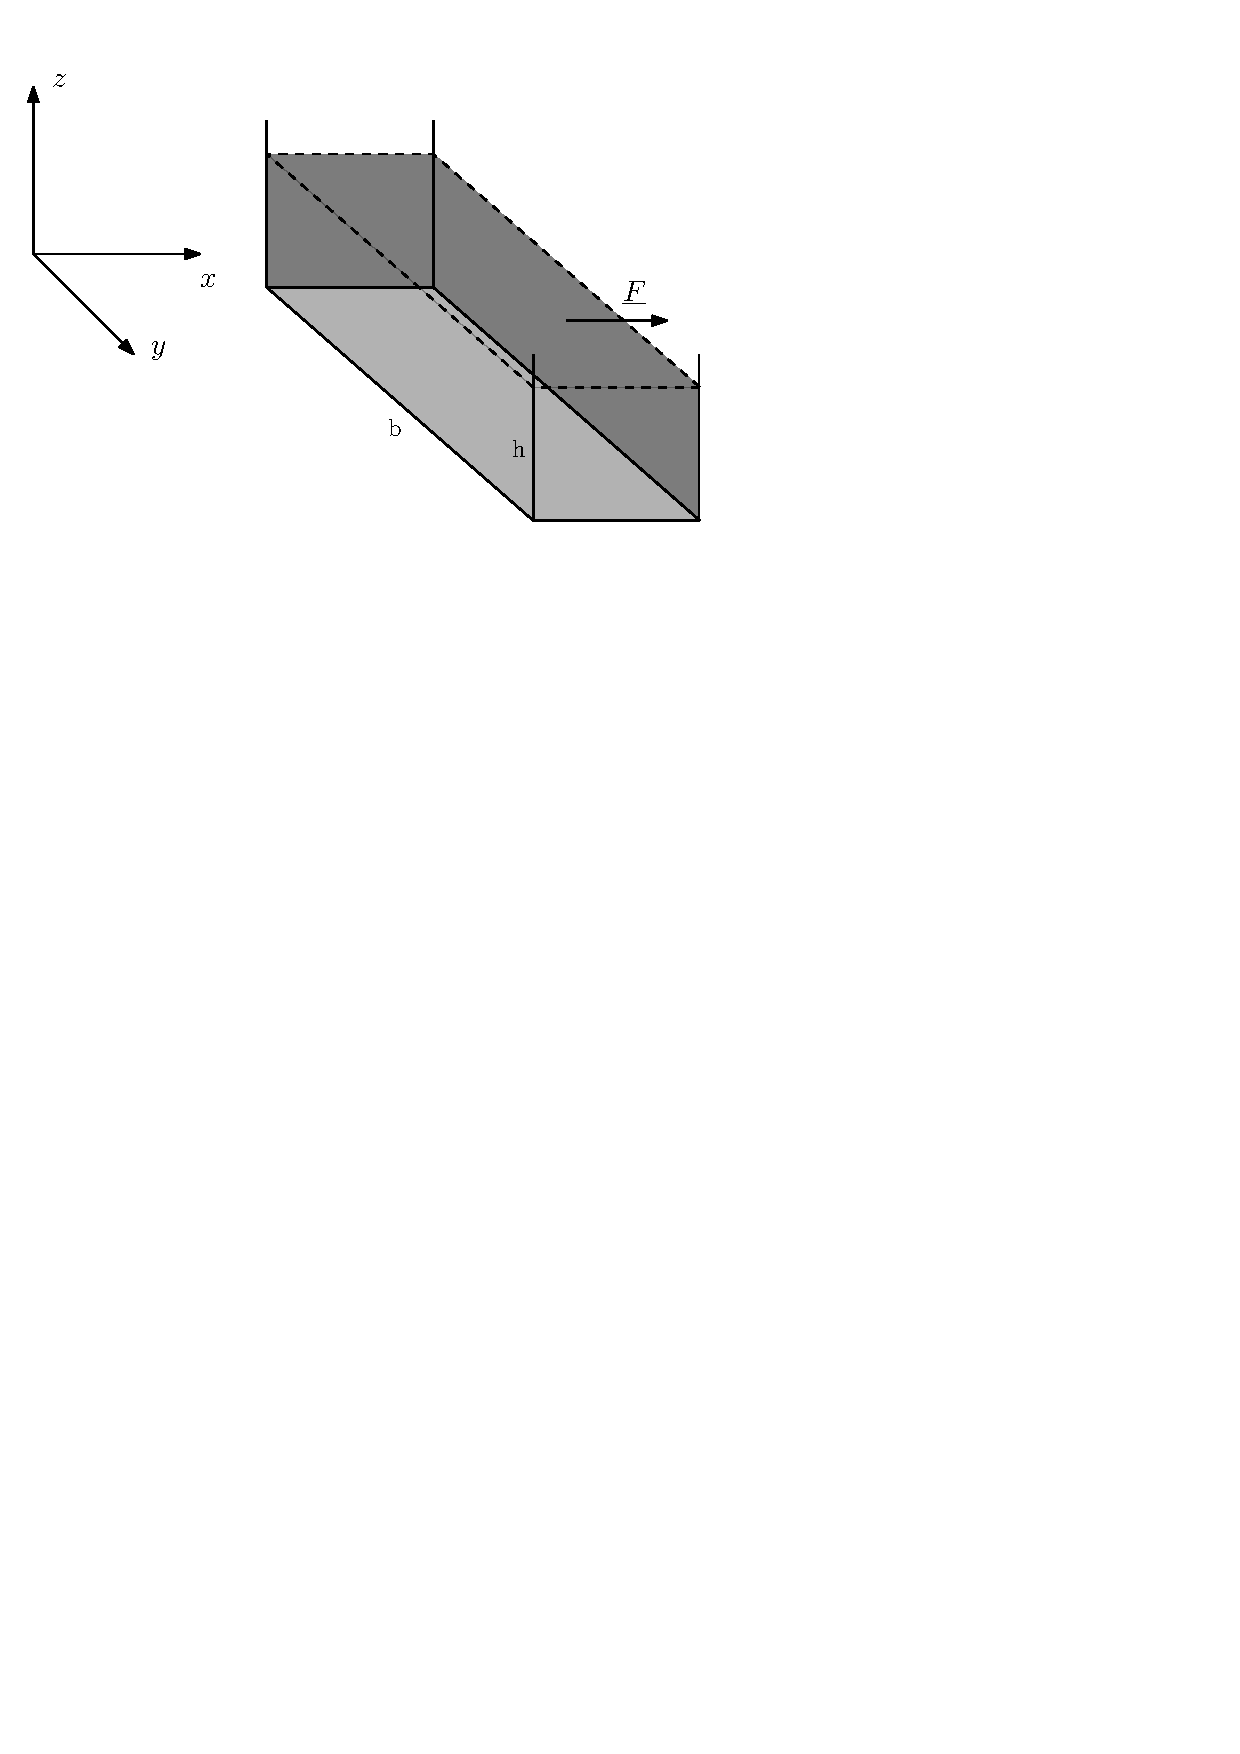
\includegraphics[scale=0.75]{./2.4 Spinte sulle superfici/2.4-3}
		\centering
		\caption{Si vuole calcolare la forza su una delle pareti laterali}
	\end{figure}
	
Partendo dalla forza come vista precedentemente:
	\begin{equation*}
		\begin{gathered}
			F = \rho g \int_0^b  \int_0^h (h - z) \dd{y} \dd{z} = \left( \rho g \right) \left( \int_0^b  \dd{y} \right) \left( \int_0^h (h - z)  \dd{z} \right) = \rho g b \frac{h^2}{2}
		\end{gathered}
	\end{equation*}
	
Notare che lo stesso risultato si sarebbe potuto ottenere con le formule relative al baricentro $b = \left( \frac{b}{2} , \frac{h}{2} \right)$:
	\begin{equation*}
		F_x = \rho g S (z_0 - z_b) = \rho g h b \left( h - \frac{h}{2} \right) = \rho g b \frac{h^2}{2}
	\end{equation*}

Oppure vedendo la forza come superficie per pressione relativa nel baricentro:
	\begin{equation*}
		F = S (p_0 - p_b) = (h b) \left(\rho g \frac{h}{2} \right) =  \rho g b \frac{h^2}{2}
	\end{equation*}

Nel calcolo della coppia invece si ha:
	\begin{equation*}
		\begin{gathered}
			\uline{r} \cross \uline{n} = \uline{r} \cross \uline{i}_x = (x, y, z) \cross (1, 0, 0) = (0, z, -y) \\
			\uline{M} = \rho g \iint (z_0 - z) (0, z, -y) \dd{y} \dd{z} \\
			\text{Questo momento ha due componenti}\\
			\uline{M}_y = \rho g \iint (z_0 -z) z \dd{y} \dd{z} = \rho g b \int_0^h (h - z) z \dd{z}  = \rho g b \frac{h^3}{6}\\
			\uline{M}_z = - \rho g \iint (z_0 - z) y \dd{y} \dd{z} = - \rho g \int_0^b y \dd{y} \int_0^h (h - z) \dd{z} = - \rho g \frac{b^2 h^2}{6}
		\end{gathered}
	\end{equation*}
	
\subsubsection{Punto di applicazione}	
Il calcolo della coppia può essere complesso, si introduce quindi il concetto di punto di applicazione, anche noto come centro di spinta.
Questo è un punto $A$ tale che applicando in esso la forza risultante del sistema ($F$), si ottiene lo stesso risultato del calcolo della coppia:
	\begin{equation*}
		\uline{r}_A : \uline{r}_A \cross \uline{F} = \uline{M}
	\end{equation*}
È quindi un modo implicito di calcolare la coppia.
Dato che questa relazione è indipendente dal polo, una volta individuato $\uline{r}_A$ si può calcolare cosa accade rispetto ad un polo qualsiasi, mentre la coppia è invece riferita ad un determinato polo.

Ad essere precisi in realtà si ha una retta di applicazione, ma sommando a $\uline{r}_A$ un vettore parallelo alla forza F il risultato non cambia, pur essendo il punto di applicazione diverso, dato che il prodotto vettoriale non cambia.

In 2D è di interesse il punto appartenente a quella retta che giace sul piano, in 3D invece un punto vale l'altro purché appartenga ad una retta parallela alla risultante $F$.

Il concetto di punto di applicazione si può introdurre anche nella meccanica dei fluidi, dato che dai momenti si può trovare il punto di applicazione a partire dal momento statico ($M_y \rightarrow z_A, M_z \rightarrow y_A$).

Ad esempio, nel caso specifico di cui prima, visto come problema in 2D, si ha questa situazione sulla parete laterale:
	\begin{figure}[ht]
		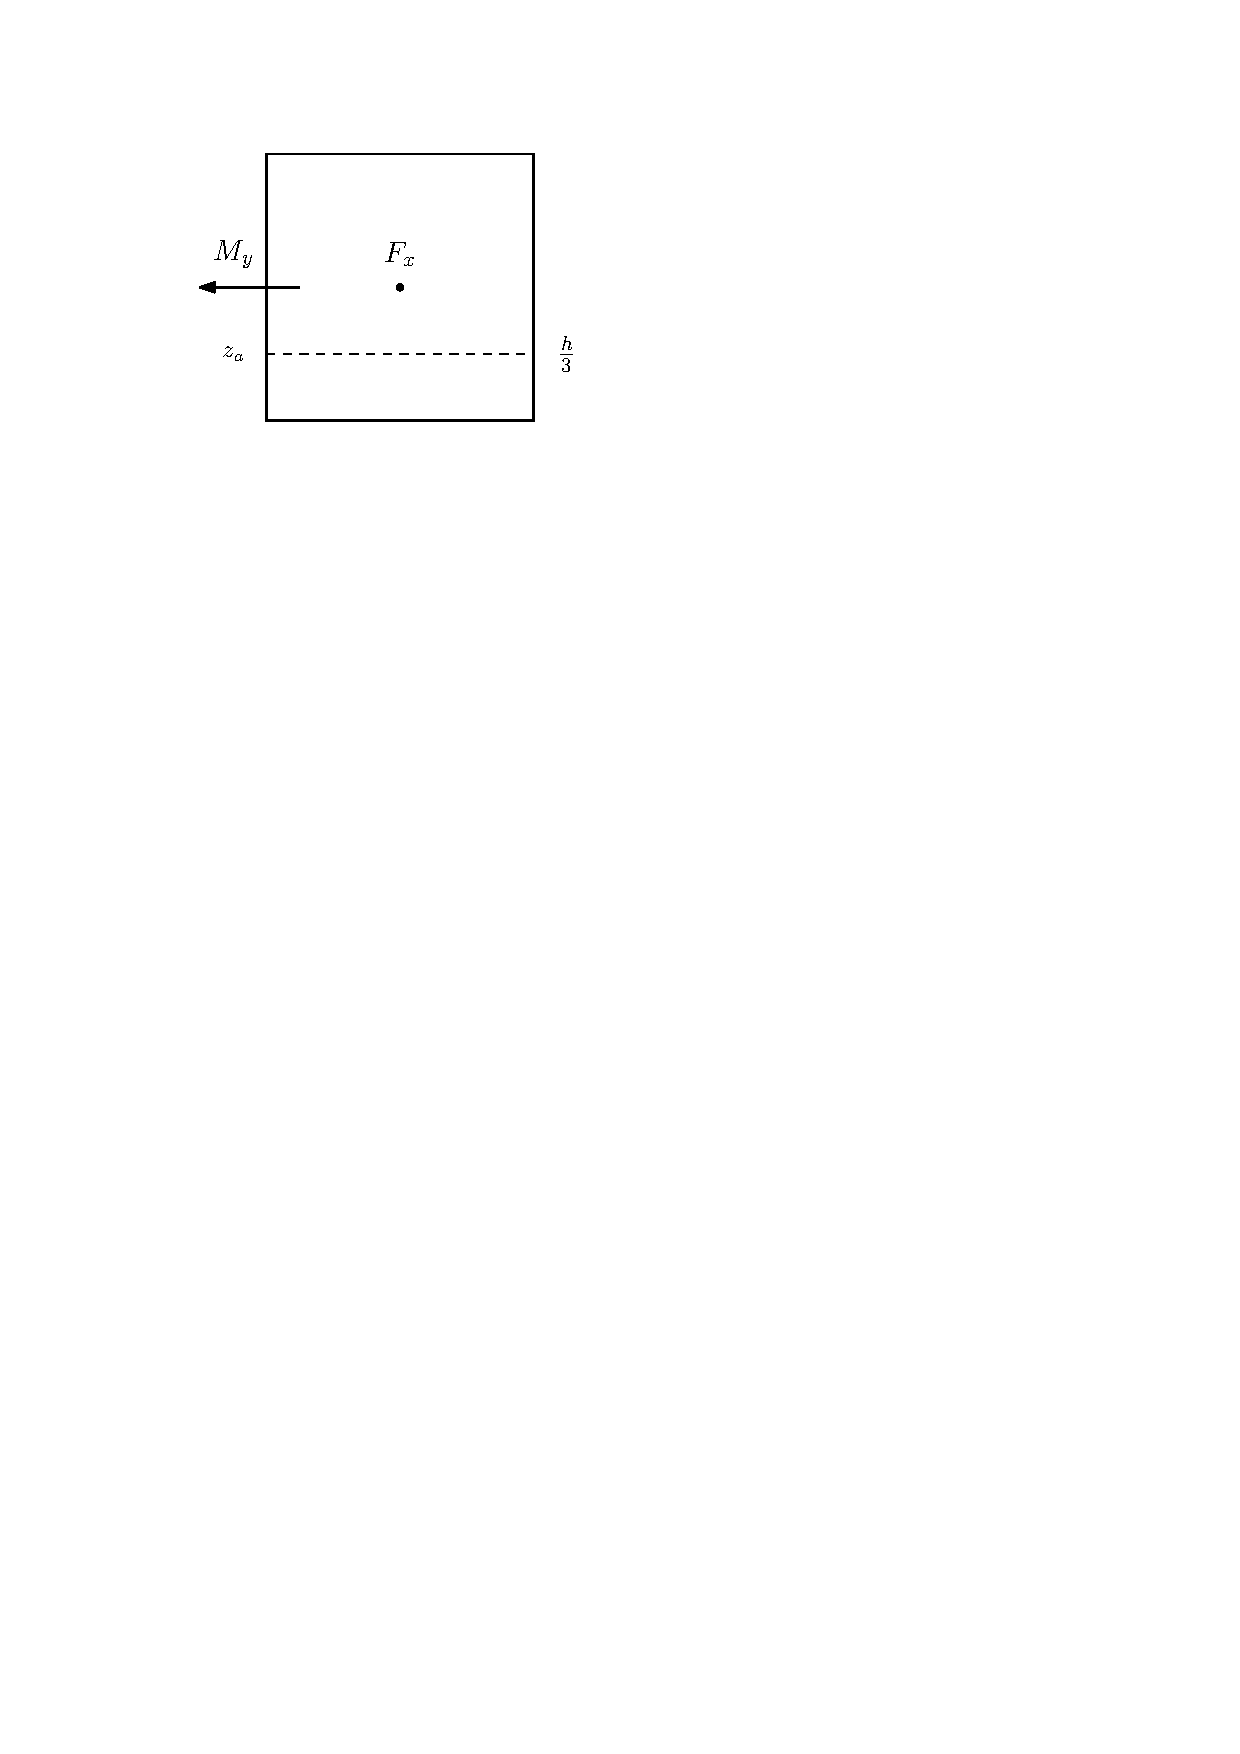
\includegraphics[scale=0.90]{./2.4 Spinte sulle superfici/2.4-4}
		\centering
		\caption{Parete laterale}
	\end{figure}	
Notare che dato che si è in un caso piano interessa solamente la forza perpendicolare ad esso, dal momento parallelo al piano si trova il punto di applicazione, in 3D sarebbe più complesso:
	\begin{equation*}
		\begin{gathered}
			M_y = z_A F_x \\
			z_A = \frac{M_y}{F_x} = \frac{\rho g b \frac{h^3}{6}}{\rho g b \frac{h^2}{2}} = \frac{h}{3}
		\end{gathered}
	\end{equation*}
È un risultato che vale per tutte le superfici piane rettangolari in cui il bordo superiore coincida con il pelo libero. Da notare che il punto di applicazione è diverso dal baricentro, che si trova a $\frac{h}{2}$.	

Come esempi si può fare riferimento a quelli di cui in \cite[Fig.\ 3.4, 3.6]{PnueliGutfinger}.
Nel primo, nel quale occorre notare che l'origine è presa nella parte superiore della figura, si dimostra che il ragionamento è analogo per una superficie obliqua.
Nel secondo, nota la direzione della forza, se ne calcola il modulo.

\subsubsection{Integrali simil-inerzia}
Negli esercizi citati in precedenza si fa riferimento a momenti d'inerzia dato che sono integrali del tipo $\int z^2 \dd{z}$, che di solito si incontrano nel calcolo dei momenti di inerzia.
È solo un artificio mnemonico per ricordare che potrebbe essere un integrale noto per via del calcolo di un momento d'inerzia per una figura di quel genere, non ha assolutamente lo stesso significato fisico.
%
\subsection{Superficie non piana e principio di Archimede}
Nel caso in cui si consideri una superficie non piana la normale non è più costante lungo la superficie, conseguentemente è una variabile all'interno degli integrali delle forze:
	\begin{equation*}
		\uline{F} = \rho g \int (z_0 -z) \uline{n} \dd{S}
	\end{equation*}
%
	\begin{figure}[ht]
		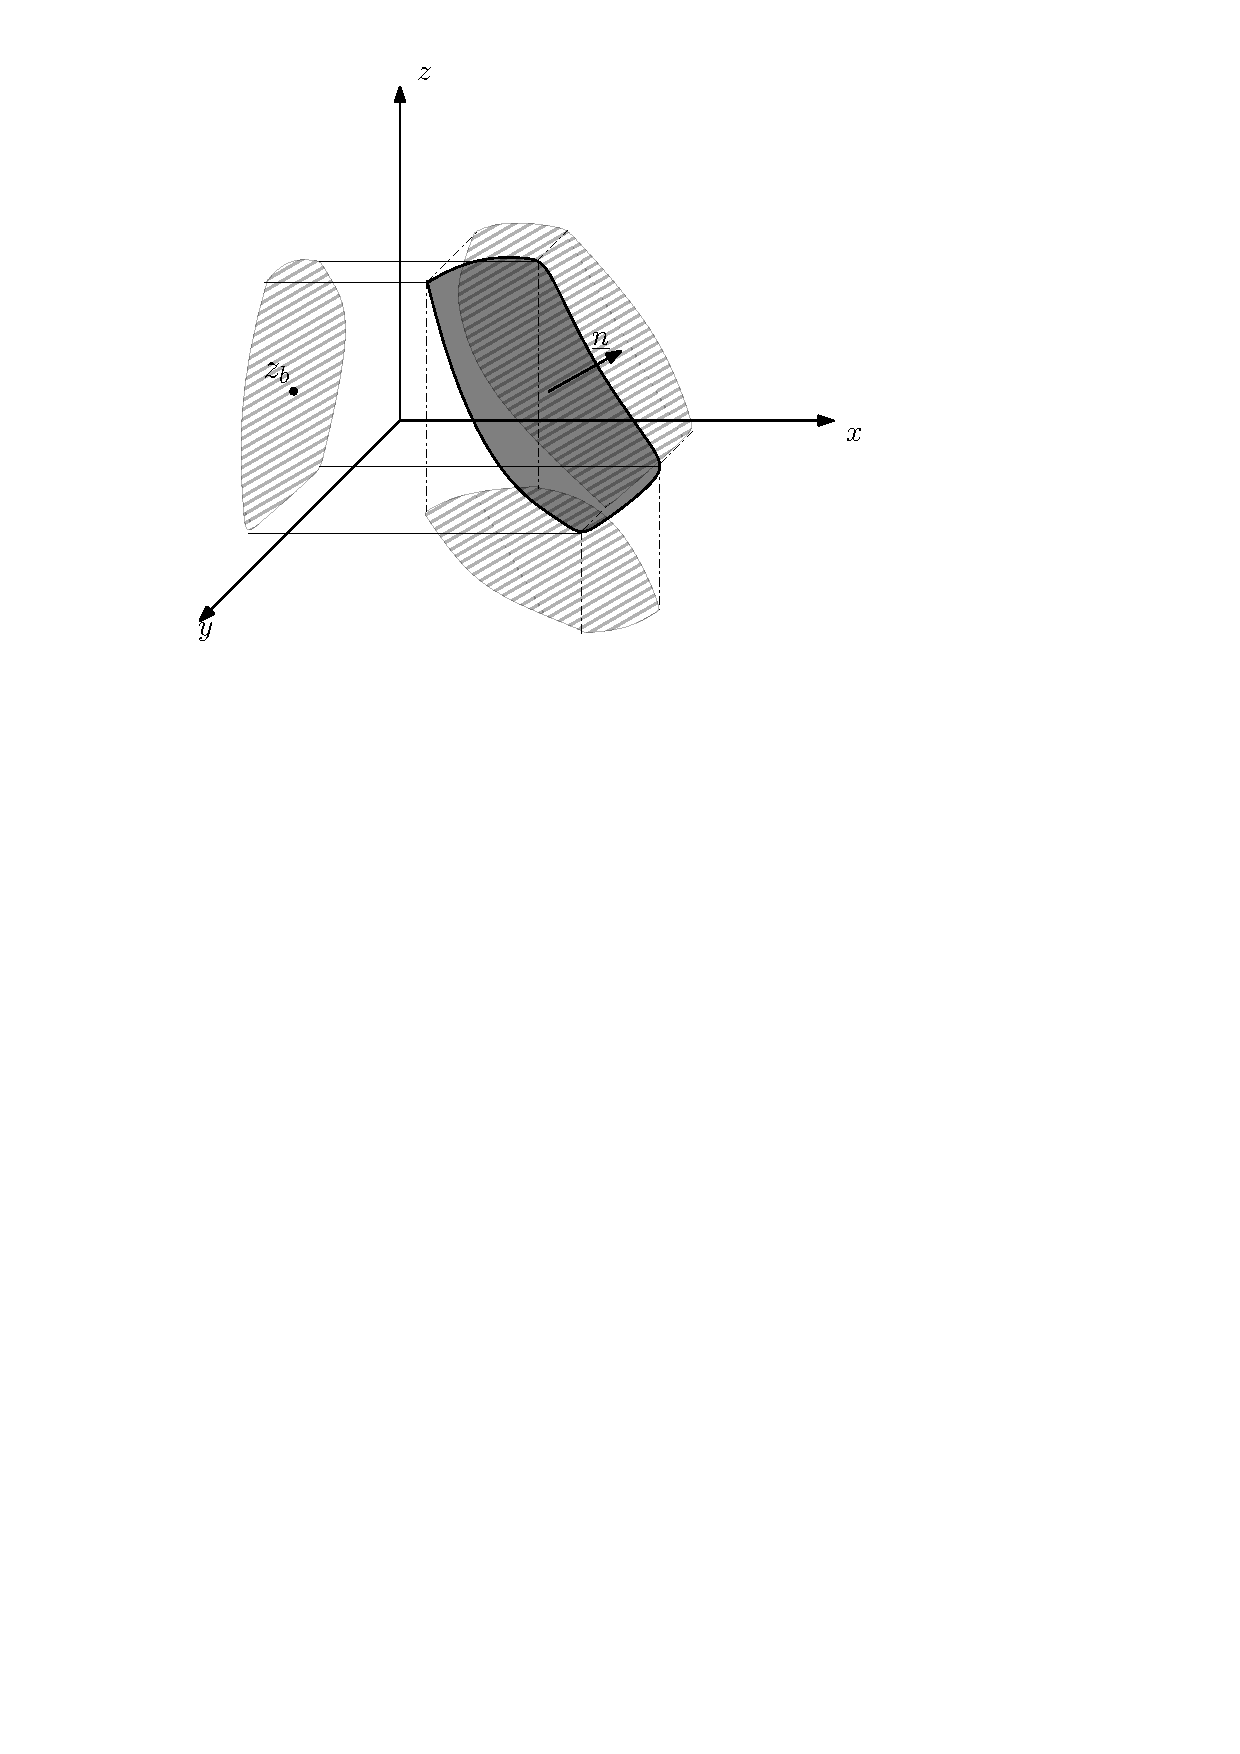
\includegraphics[scale=1.10]{./2.4 Spinte sulle superfici/2.4-5}
		\centering
		\caption{Superficie non piana e proiezioni}
	\end{figure}	
Si considera quindi una componente alla volta ed in questo risulta utile ricordare che:
	\begin{equation*}
		\uline{n} \dd{S} = (\pm \dd{y} \dd{z}, \pm \dd{x} \dd{y}, \pm \dd{x} \dd{y})
	\end{equation*}
%
Ne derivano tre integrali relativamente semplici, in cui il segno dipende da se la normale sia concorde/discorde con l'asse in esame, ad esempio supponendo di avere la normale positiva lungo l'asse x:
	\begin{equation*}
		\begin{gathered}
			F_x = \rho g \int_{S_{yz}} (z_0 - z) \dd{y} \dd{z} = (p_0 - p_b) S_{yz}\footnote{b è il baricentro della proiezione} \\
			F_y = \rho g \int_{S_{xz}} (z_0 - z) \dd{x} \dd{z} = (p_0 - p_b) S_{xz}\footnote{b è il baricentro della proiezione} \\
			F_z = \rho g \int (z_0 - z) \dd{x} \dd{y}
		\end{gathered}
	\end{equation*}
In questo esempio il primo integrale è la proiezione della superficie S sul piano yz, è come il caso della superficie piana, nel secondo invece la proiezione è sul piano xz e analogamente ci si riconduce al caso di superficie piana.
Nel terzo, avendo z per la superficie $\dd{x} \dd{y}$, l'integrale  rappresenta il volume dell'oggetto compreso tra la superficie e la proiezione, che è una informazione interessante.
Le componenti orizzontali della forza si calcolano quindi con formule della superficie piana applicate a proiezioni diverse, la componente verticale è invece correlata al volume compreso tra la superficie e la sua proiezione, interessante nel caso di una superficie chiusa.	
Notare che in questi integrali la normale non varia lungo la superficie, ci si è ricondotti al caso piano calcolando gli integrali sulle proiezioni.

Tornando all'integrale sul piano xy, questo rappresenta il volume dell'oggetto compreso tra la superficie e la sua proiezione. Particolarizzando nel caso di una superficie chiusa vediamo che si hanno un contributo ``positivo'' ed uno ``negativo'':
	\begin{figure}[ht]
		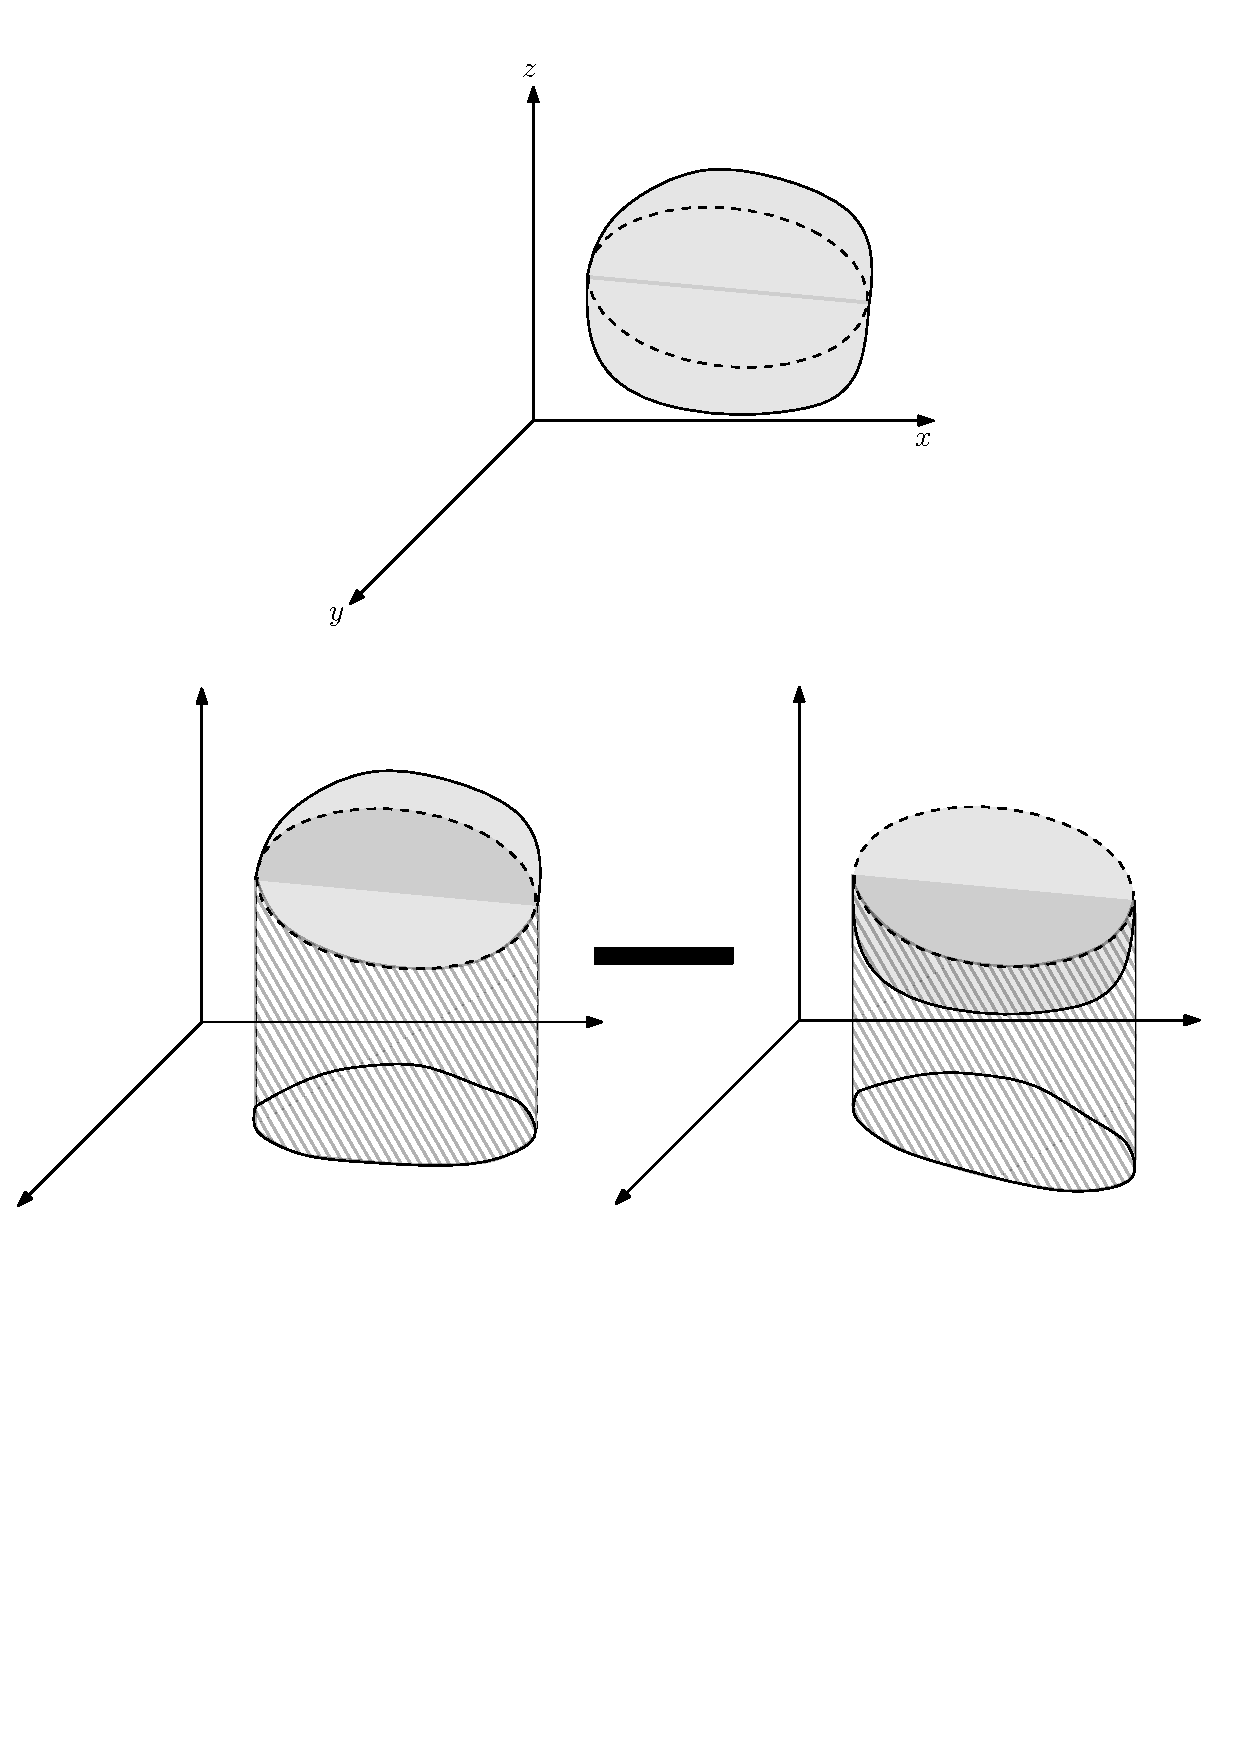
\includegraphics[scale=0.60]{./2.4 Spinte sulle superfici/2.4-6}
		%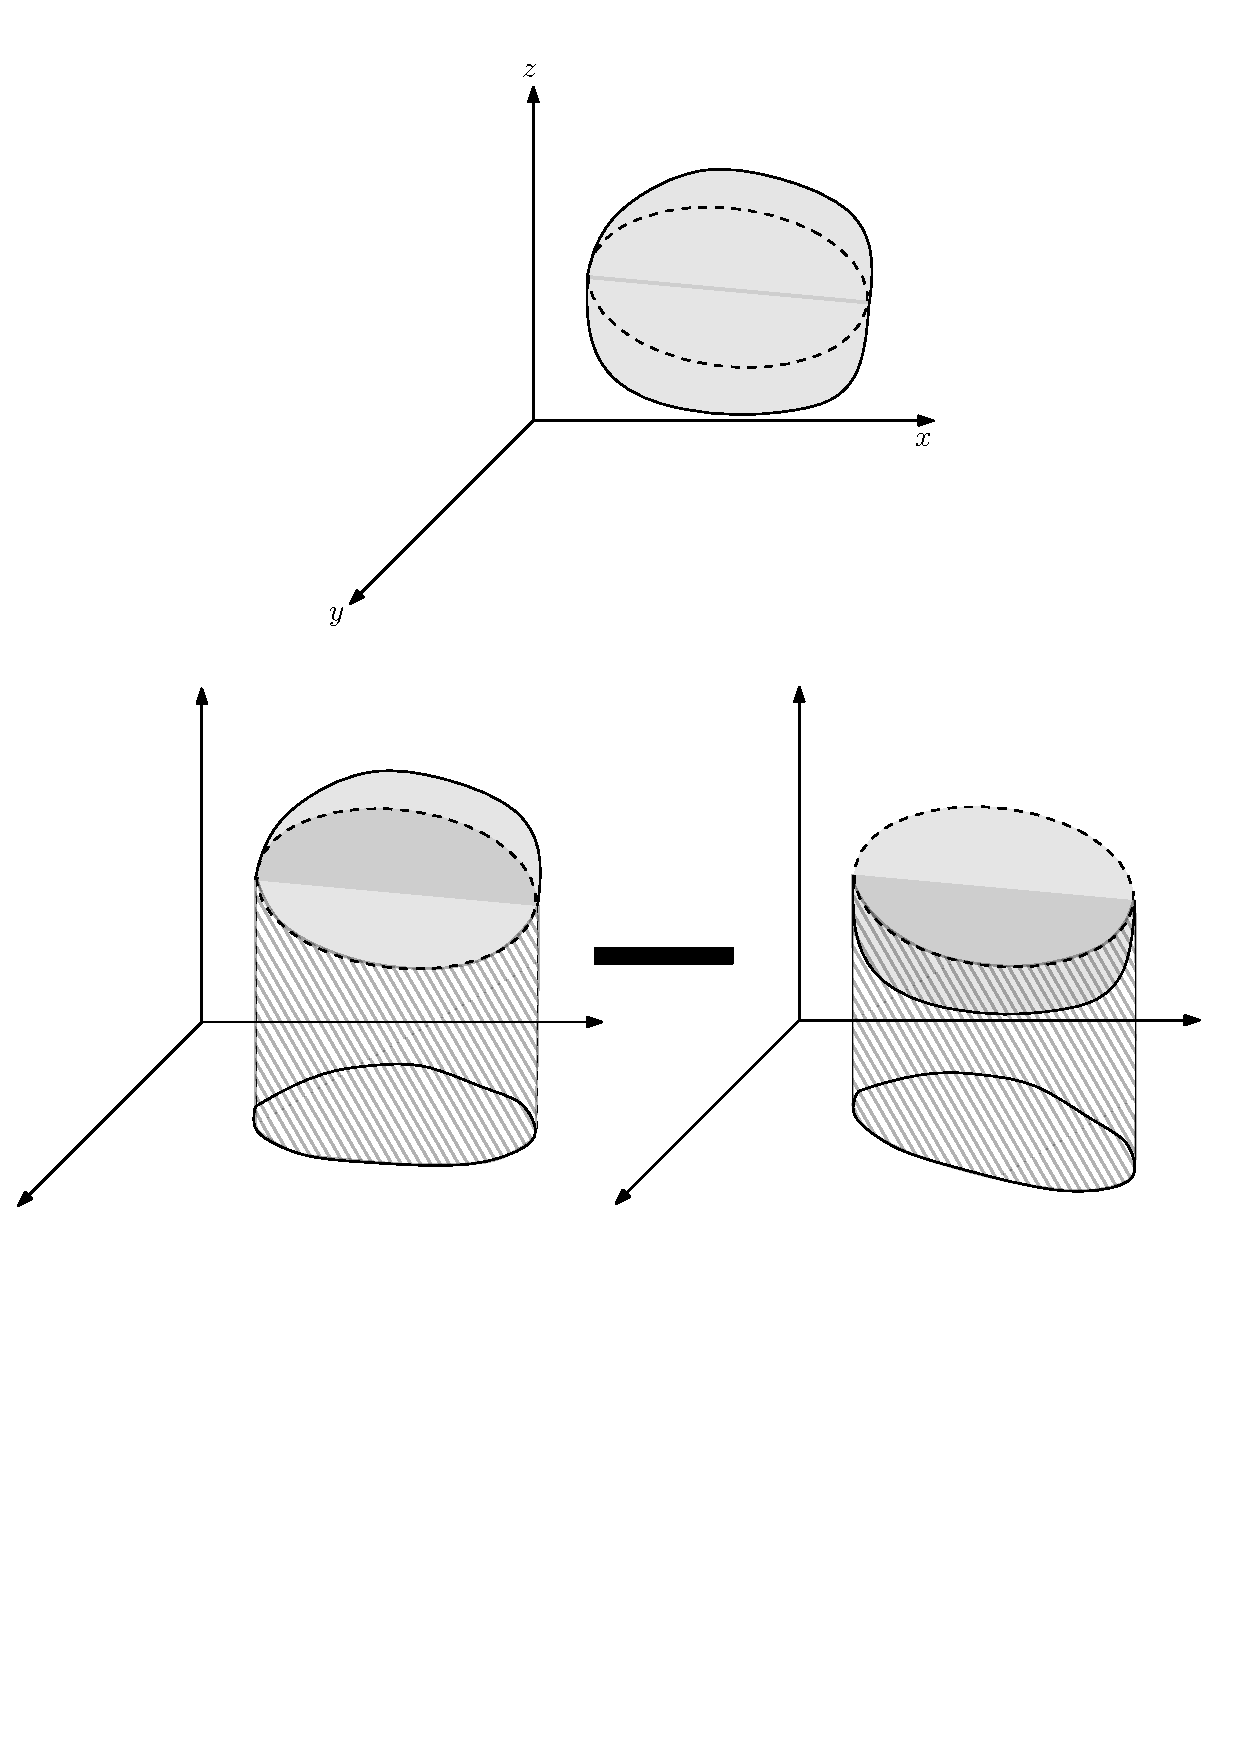
\includegraphics[width=\textwidth,height=\textheight,keepaspectratio]{./2.4 Spinte sulle superfici/2.4-6}
		\centering
		\caption{Sommando si ottiene il volume racchiuso dalla superficie chiusa}
	\end{figure}
Una metà ha componente positiva lungo z, l'altra metà negativa, sommandole si ottiene il volume racchiuso dalla superficie di partenza.
L'espressione della forza lungo z di conseguenza diventa:
	\begin{equation*}
		F_z = \rho g V_S \quad \textbf{Principio di Archimede}
	\end{equation*}
In questa $\rho V_S$ rappresenta la massa del fluido contenuto nella superficie S, per g diventa una forza peso, questo termine è noto nel principio di Archimede come ``peso del volume di liquido spostato''.
Le forze lungo gli altri due assi, nel caso in cui la superficie chiusa sia ``in orizzontale'' saranno nulle dato che i due contributi al volume avranno lo stesso baricentro, dando quindi contributi uguali ma di segno opposto, la cui somma è nulla.		
Nel caso di superficie aperta si possono invece avere tutte e tre le componenti.
	
\subsection*{Bibliografia 2.4}
\cite[Cap.\ 3.4, 3.5, 3.6, 3.7]{CengelCimbala}\\
\cite[Cap.\ 3.4, 3.5, 3.6]{PnueliGutfinger}